% Author Alfredo Sánchez Alberca (asalber@ceu.es)

\newproblem{vac-1}{gen}{}
%ENUNCIADO
{Una variable aleatoria continua $X$ tiene una función de densidad dada por:
\[
f(x)=
\begin{cases}
k(6-3x) & \text{si $0\leq x\leq 2$,} \\
0 & \text{si  $x<0$ o $x>2$.}
\end{cases}
\]
\begin{enumerate}
\item  Determinar el valor de $k$.
\item  Hallar $P(X\leq 1)$; $P(X>2)$; $P(X=1/4)$; $P(1/3\leq X\leq 2/3)$.
\item  Calcular $\mu$ y $\sigma$.
\item  Hallar la función de distribución $F(x)$.
\end{enumerate}
}
%SOLUCIÓN
{
\begin{enumerate}
\item $k=1/6$.
\item $P(X\leq 1)=0.75$, $P(X>2)=0$, $P(X=1/4)=0$ y $P(1/3\leq X\leq 2/3)=1/4$.
\item $\mu=2/3$, $\sigma^2=2/9$ y $\sigma=\sqrt{2}/3$.
\item \[
F(x)=
\begin{cases}
0 & \text{si $x<0$,}\\
x-\frac{x^2}{4} & \text{si $0\leq x\leq 2$,}\\
1 & \text{si $2<x$.}
\end{cases}
\]
\end{enumerate}
}
%RESOLUCIÓN
{}


\newproblem{vac-2}{gen}{*}
%ENUNCIADO
{La función de densidad de la variable aleatoria continua $X$ viene dada por la gráfica siguiente:
\begin{center}
\scalebox{0.6}{% Created by tikzDevice version 0.10.1 on 2016-11-03 09:31:09
% !TEX encoding = UTF-8 Unicode
\begin{tikzpicture}[x=1pt,y=1pt]
\definecolor{fillColor}{RGB}{255,255,255}
\path[use as bounding box,fill=fillColor,fill opacity=0.00] (0,0) rectangle (289.08,289.08);
\begin{scope}
\path[clip] ( 42.00, 42.00) rectangle (277.08,253.08);
\definecolor{drawColor}{RGB}{5,161,230}

\path[draw=drawColor,line width= 0.8pt,line join=round,line cap=round] ( 50.71, 42.00) --
	(159.54,217.90) --
	(268.37, 42.00);
\end{scope}
\begin{scope}
\path[clip] (  0.00,  0.00) rectangle (289.08,289.08);
\definecolor{drawColor}{RGB}{0,0,0}

\path[draw=drawColor,line width= 0.4pt,line join=round,line cap=round] ( 50.71, 42.00) -- (268.37, 42.00);

\path[draw=drawColor,line width= 0.4pt,line join=round,line cap=round] ( 50.71, 42.00) -- ( 50.71, 36.00);

\path[draw=drawColor,line width= 0.4pt,line join=round,line cap=round] (105.12, 42.00) -- (105.12, 36.00);

\path[draw=drawColor,line width= 0.4pt,line join=round,line cap=round] (159.54, 42.00) -- (159.54, 36.00);

\path[draw=drawColor,line width= 0.4pt,line join=round,line cap=round] (213.96, 42.00) -- (213.96, 36.00);

\path[draw=drawColor,line width= 0.4pt,line join=round,line cap=round] (268.37, 42.00) -- (268.37, 36.00);

\node[text=drawColor,anchor=base,inner sep=0pt, outer sep=0pt, scale=  1.00] at ( 50.71, 25.20) {0.0};

\node[text=drawColor,anchor=base,inner sep=0pt, outer sep=0pt, scale=  1.00] at (105.12, 25.20) {0.5};

\node[text=drawColor,anchor=base,inner sep=0pt, outer sep=0pt, scale=  1.00] at (159.54, 25.20) {1.0};

\node[text=drawColor,anchor=base,inner sep=0pt, outer sep=0pt, scale=  1.00] at (213.96, 25.20) {1.5};

\node[text=drawColor,anchor=base,inner sep=0pt, outer sep=0pt, scale=  1.00] at (268.37, 25.20) {2.0};

\path[draw=drawColor,line width= 0.4pt,line join=round,line cap=round] ( 42.00, 42.00) -- ( 42.00,253.08);

\path[draw=drawColor,line width= 0.4pt,line join=round,line cap=round] ( 42.00, 42.00) -- ( 36.00, 42.00);

\path[draw=drawColor,line width= 0.4pt,line join=round,line cap=round] ( 42.00, 77.18) -- ( 36.00, 77.18);

\path[draw=drawColor,line width= 0.4pt,line join=round,line cap=round] ( 42.00,112.36) -- ( 36.00,112.36);

\path[draw=drawColor,line width= 0.4pt,line join=round,line cap=round] ( 42.00,147.54) -- ( 36.00,147.54);

\path[draw=drawColor,line width= 0.4pt,line join=round,line cap=round] ( 42.00,182.72) -- ( 36.00,182.72);

\path[draw=drawColor,line width= 0.4pt,line join=round,line cap=round] ( 42.00,217.90) -- ( 36.00,217.90);

\path[draw=drawColor,line width= 0.4pt,line join=round,line cap=round] ( 42.00,253.08) -- ( 36.00,253.08);

\node[text=drawColor,anchor=base east,inner sep=0pt, outer sep=0pt, scale=  1.00] at ( 34.80, 38.56) {0.0};

\node[text=drawColor,anchor=base east,inner sep=0pt, outer sep=0pt, scale=  1.00] at ( 34.80, 73.74) {0.2};

\node[text=drawColor,anchor=base east,inner sep=0pt, outer sep=0pt, scale=  1.00] at ( 34.80,108.92) {0.4};

\node[text=drawColor,anchor=base east,inner sep=0pt, outer sep=0pt, scale=  1.00] at ( 34.80,144.10) {0.6};

\node[text=drawColor,anchor=base east,inner sep=0pt, outer sep=0pt, scale=  1.00] at ( 34.80,179.28) {0.8};

\node[text=drawColor,anchor=base east,inner sep=0pt, outer sep=0pt, scale=  1.00] at ( 34.80,214.46) {1.0};

\node[text=drawColor,anchor=base east,inner sep=0pt, outer sep=0pt, scale=  1.00] at ( 34.80,249.64) {1.2};

\path[draw=drawColor,line width= 0.4pt,line join=round,line cap=round] ( 42.00, 42.00) --
	(277.08, 42.00) --
	(277.08,253.08) --
	( 42.00,253.08) --
	( 42.00, 42.00);
\end{scope}
\begin{scope}
\path[clip] (  0.00,  0.00) rectangle (289.08,289.08);
\definecolor{drawColor}{RGB}{0,0,0}

\node[text=drawColor,anchor=base,inner sep=0pt, outer sep=0pt, scale=  1.00] at (159.54,  6.00) {X};

\node[text=drawColor,rotate= 90.00,anchor=base,inner sep=0pt, outer sep=0pt, scale=  1.00] at ( 13.20,147.54) {Densidad de probabilidad $f(x)$};
\end{scope}
\begin{scope}
\path[clip] ( 42.00, 42.00) rectangle (277.08,253.08);
\definecolor{drawColor}{RGB}{190,190,190}

\path[draw=drawColor,line width= 0.4pt,dash pattern=on 4pt off 4pt ,line join=round,line cap=round] ( 50.71, 42.00) -- ( 50.71,217.90);

\path[draw=drawColor,line width= 0.4pt,dash pattern=on 4pt off 4pt ,line join=round,line cap=round] (159.54, 42.00) -- (159.54,217.90);
\end{scope}
\end{tikzpicture}
}
\end{center}
Calcular:
\begin{enumerate}
\item $P(\frac{1}{2}\leq X\leq \frac{5}{4})$.
\item Función de distribución.
\item Media y desviación típica.
\end{enumerate}
}
%SOLUCIÓN
{
\begin{enumerate}
\item $P(\frac{1}{2}\leq X\leq \frac{5}{4})=19/32$.
\item \[
F(x)=
\begin{cases}
0 & \text{si $x<0$,}\\
\frac{x^2}{2} & \text{si $0\leq x\leq 1$,}\\
-\frac{x^2}{2}+2x-1 & \text{si $1<x\leq 2$,}\\
1 & \text{si $2<x$.}
\end{cases}
\]
\item $\mu=1$, $\sigma^2=1/6$ y $\sigma=1/\sqrt{6}$.
\end{enumerate}
}
%RESOLUCIÓN
{}


\newproblem*{vac-3}{gen}{*}
%ENUNCIADO
{Dada la función de densidad dada por la siguiente gráfica,
\begin{center}
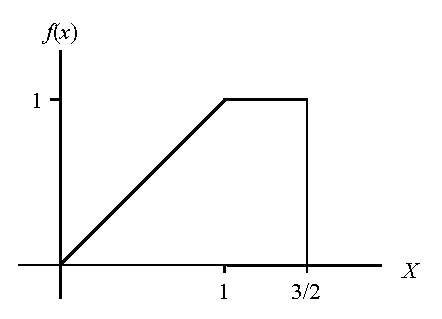
\includegraphics[scale=0.8]{img/vac-3}
\end{center}
calcular:

\begin{enumerate}
\item $P(X<1)$, $P(X>0)$, $P(X=1/4)$, $P(1/2\leq X\leq 3/2)$.
\item Media y desviación típica.
\end{enumerate}
}
%SOLUCIÓN
{}
%RESOLUCIÓN
{}


\newproblem{vac-4}{amb}{*}
%ENUNCIADO
{Se sabe que la duración de las baterías de un tipo de marcapasos (expresada en años) es una variable aleatoria cuya
función de densidad es
\[
f(x)=
\begin{cases}
0 & \text{si $x<0$,}\\
\dfrac{e^{-x/10}}{10} & \text{si $x\geq 0$.}
\end{cases}
\]
Se pide:
\begin{enumerate}
\item Comprobar que $f(x)$ es función de densidad.
\item Calcular la función de distribución.
\item Calcular la probabilidad de que la batería dure menos de 5 años, y de que dure entre 5 y 10 años.
\item Calcular la vida media de la batería.
\end{enumerate}
}
%SOLUCIÓN
{
\begin{enumerate}
\item $\int_{-\infty}^\infty f(x)\, dx = [-e^{-x/10}]_{-\infty}^\infty = 1$.
\item \[
F(x)=
\begin{cases}
0 & \text{si $s<0$,}\\
1-e^{-x/10} & \text{si $x\geq 0$.}
\end{cases}
\]
\item $P(X<5)=0.3935$ y $P(5<X<10)=0.2387$.
\item $\mu=10$ años.
\end{enumerate}
}
%RESOLUCIÓN
{}


\newproblem*{vac-5}{amb}{*}
% ENUNCIADO
{La proporción de cierto aditivo en la gasolina determina su precio. Si en la producción de gasolina la proporción de
aditivo es una variable aleatoria $X$ con función de densidad $f(x)=6x(1-x)$ para $0\leq x\leq 1$, de manera que si
$x<0,5$ la gasolina es del tipo I y se vende a $0.6$ \euro/l, si $0.5\leq x\leq 0.8$ la gasolina es del tipo II y se
vende a $0.7$ \euro/l, y si $x>0.8$ la gasolina es del tipo III que se vende a $0.8$ \euro/l, se pide:
\begin{enumerate}
\item Calcular la función de distribución de $X$.
\item Calcular los porcentajes de producción de cada tipo de gasolina.
\item Calcular el precio medio por litro.
\end{enumerate}
}
%SOLUCIÓN
{}
%RESOLUCIÓN
{}


\newproblem{vac-6}{gen}{}
%ENUNCIADO
{Un empleado suele acudir al trabajo en cualquier instante entre las 6 y las 7 con igual probabilidad. Se pide:
\begin{enumerate}
\item Calcular la función de densidad de la variable que mide el instante en que acude a trabajar y dibujarla.
\item Calcular la función de distribución y dibujarla.
\item Calcular la probabilidad de que llegue entre las 6 y cuarto y las 6 y media.
\item Calcular la hora media a la que se espera que llegue.
\end{enumerate}
}
%SOLUCIÓN
{
\begin{enumerate}
\item \[
f(x)=
\begin{cases}
0 & \text{si $x<6$,}\\
1 & \text{si $6\leq x\leq 7$,}\\
0 & \text{si $7<x$.}
\end{cases}
\]
\item \[
F(x)=
\begin{cases}
0 & \text{si $x<6$,}\\
x-6 & \text{si $6\leq x\leq 7$,}\\
1 & \text{si $7<x$.}
\end{cases}
\]
\item $P(6.25<X<6.5)=0.25$.
\item $\mu=6.5$, es decir, a las 6 horas y media.
\end{enumerate}
}
%RESOLUCIÓN
{}


\newproblem{vac-7}{gen}{}
%ENUNCIADO
{Sea $Z$ una variable aleatoria que sigue una distribución $N(0,1)$.
Determinar el valor de $t$ en cada uno de los siguientes casos: 
\begin{enumerate}
\item El área entre $0$ y $t$ es $0.4783$.
\item El área a la izquierda de $t$ es $0.6406$.
\item El área entre $-1.5$ y $t$ es $0.2313$.
\end{enumerate}
}
%SOLUCIÓN
{
\begin{enumerate}
\item $t=2.02$.
\item $t=0.36$.
\item $t=-0.53$.
\end{enumerate}
}
%RESOLUCIÓN
{}


\newproblem*{vac-8}{gen}{}
%ENUNCIADO
{Hallar las siguientes probabilidades:

\begin{enumerate}
\item  $P(-2.4$ $\leq Z\leq -1.2)$ si $Z$ es $N(0,1)$.
\item  $P(\left| Z\right| >1.2)$ si $Z$ es $N(0,1)$.
\item  $P(1.3\leq X\leq 3.3)$ si $X$ es $N(2,1)$.
\item  $P(\left| X-3\right| >2)$ si $X$es $N(3,4)$.
\end{enumerate}
}
%SOLUCIÓN
{}
%RESOLUCIÓN
{}


\newproblem*{vac-9}{gen}{*}
%ENUNCIADO
{Supongamos una variable aleatoria $X$ que sigue una distribución normal de desviación típica 1 ($\sigma =1)$, y media ($\mu )$ desconocida. Si nos dan como dato que la función de densidad en $x$=1 vale $\dfrac{1}{\sqrt{2\pi }},$ y teniendo en cuenta que la función de densidad viene dada por:
\[
f(x)=\dfrac{1}{\sigma \sqrt{2\pi }}\ e^{-\dfrac{(x-\mu )^{2}}{2\sigma ^{2}}},
\]
calcular $P(\left| X-2\right| <3)$.
}
%SOLUCIÓN
{}
%RESOLUCIÓN
{}


\newproblem{vac-10}{med}{}
%ENUNCIADO
{Se sabe que el nivel de colesterol en varones de más de 30 años sigue una distribución normal, de media 220 mg/dl y desviación típica 30 mg/dl. Realizando un estudio sobre 20000 varones mayores de 30 años,
\begin{enumerate}
\item ¿Cuántos se espera que tengan su nivel de colesterol entre 210 y 240 mg/dl?
\item Si un nivel de colesterol por encima de 250 mg/dl puede provocar trombosis, ¿cuántos tienen riesgo de trombosis?
\item ¿Cuál será el nivel de colesterol por encima del cual está el 20\% de la población?
\end{enumerate}
}
%SOLUCIÓN
{
\begin{enumerate}
\item $P(210\leq X\leq 240)=0.3781\rightarrow 7561.3$  varones. 
\item $P(X>250)=0.1587\rightarrow 3173.1$ varones. 
\item $P_{80}=245.2486$ mg/dl. 
\end{enumerate}
}
%RESOLUCIÓN
{}


\newproblem{vac-11}{med}{}
%ENUNCIADO
{Entre los diabéticos, el nivel de glucosa en la sangre en ayunas, puede suponerse de distribución aproximadamente
normal, con media 106 mg/100 ml y desviación típica 8 mg/100 ml.
\begin{enumerate}
\item Calcular la probabilidad de que una persona diabética elegida al azar tenga un nivel de glucosa inferior a  120mg/100ml.
\item ¿Qué porcentaje de diabéticos tendrá niveles entre 90 y 120 mg/100 ml?
\item Calcular e interpretar el primer cuartil del nivel de glucosa. 
\end{enumerate}
}
%SOLUCIÓN
{
\begin{enumerate}
\item $P(X\leq 120)=0.9599$.
\item $P(90< X<120)=0.9371$, es decir, un $93.71\%$.
\item $100.64$ mg/$100$ ml. 
\end{enumerate}
}
%RESOLUCIÓN
{}


\newproblem*{vac-12}{gen}{}
%ENUNCIADO
{Se sabe que la distribución de probabilidad de una variable aleatoria $X$ sigue la ley normal. Si conocemos $P(X>3.6)=0.3821$ y $P(X<5.8)=0.9192$, calcular $\mu $ y $\sigma $ de la distribución normal.
}
%SOLUCIÓN
{}
%RESOLUCIÓN
{}


\newproblem{vac-13}{med}{}
%ENUNCIADO
{En una población con 40000 personas, se sabe que 2276 tienen entre 0.80 y 0.84 miligramos de bilirrubina por decilitro
de sangre, y que 11508 tienen más de 0.84.
Suponiendo que la concentración de bilirrubina en sangre sigue una distribución normal, se pide:  
\begin{enumerate}
\item Calcular su media y su desviación típica.
\item Calcular el número de personas con más de 1 miligramo de bilirrubina por decilitro de sangre.
\end{enumerate}
}
%SOLUCIÓN
{
\begin{enumerate}
\item $\mu=0.7$ mg y $\sigma=0.25$ mg.
\item $P(X>1)=0.1151$ y el número de personas con más de 1 mg de bilirrubina es $0.1151\cdot 40000=4604$.
\end{enumerate}
}
%RESOLUCIÓN
{}


\newproblem{vac-14}{gen}{*}
%ENUNCIADO
{En un examen, el 63\% de los alumnos ha obtenido una nota superior a 5, y el 44\% entre 5 y 7.
Suponiendo que las notas siguen una distribución normal:

\begin{enumerate}
\item  Calcular la media y la desviación típica de las notas.
\item  Calcular el porcentaje de alumnos con nota superior a 8.
\item  ¿Cuál es la nota por encima de la cual está el 5\% de los alumnos?
\end{enumerate}
}
%SOLUCIÓN
{Llamando $X$ a la nota obtenida en el examen, se tiene que $X\sim N(\mu,\sigma)$.
\begin{enumerate}
\item $\mu=5.55$ puntos y $\sigma=1.65$ puntos.
\item $P(X>8)=0.0648$, es decir, el $6.48\%$ de los alumnos han tenido una nota superior a 8.
\item $8.21$ puntos.
\end{enumerate}
}
%RESOLUCIÓN
{}


\newproblem*{vac-15}{med}{*}
%ENUNCIADO
{Se realiza un estudio sobre la tensión arterial máxima en varones de edad comprendida entre 30 y 40 años. Como
consecuencia del estudio se sabe que el 40\% la tiene por encima de 140 mmHg y el 20\% por debajo de 110 mmHg.
Suponiendo que la tensión arterial máxima sigue una distribución normal, se pide:
\begin{enumerate}
\item Calcular la media y la desviación típica.
\item Calcular el porcentaje de hipertensos, si se considera hipertenso a una persona cuya tensión arterial máxima sea mayor que 150 mmHg.
\item ¿Cuál es el valor de la tensión arterial máxima por encima del cual se espera que esté el 10\% de la población?
\end{enumerate}
}
%SOLUCIÓN
{}
%RESOLUCIÓN
{}


\newproblem{vac-16}{gen}{*}
%ENUNCIADO
{Un grupo de 100 alumnos realiza un examen. Una vez corregido, el profesor observa que la nota media es $4.2$ y que 32 alumnos han tenido una calificación superior a $5$. Suponiendo que las notas siguen una distribución normal, ¿cuántos alumnos habrán obtenido una calificación superior a $7$?
}
%SOLUCIÓN
{$P(X>7)=0.0508\rightarrow 5.1$ alumnos.
}
%RESOLUCIÓN
{}


\newproblem{vac-17}{med}{*}
%ENUNCIADO
{Se supone que la tensión arterial de los habitantes de una población de 20000 habitantes sigue una distribución
normal, cuya media es 13 y su rango intercuartílico 4.
Se pide:
\begin{enumerate}
\item ¿Cuántas personas tienen una tensión por encima de 16?
\item ¿Cuánto tendrá que disminuir la tensión de una persona que tiene 16 para situarse en el 40\% de la población con
tensión más baja?
\end{enumerate}
}
%SOLUCIÓN
{
\begin{enumerate}
\item $P(X>16)=0.1587$ y el número de personas con tensión por encima de 16 mmHg es $0.1587\cdot 20000=3174$.
\item Debe disminuir $3.75$ mmHg.
\end{enumerate}
}
%RESOLUCIÓN
{}


\newproblem{vac-18}{med}{*}
%ENUNCIADO
{En una población de 30000 individuos se está interesado en medir el volumen sanguíneo de sus individuos.
Se sabe que la desviación típica de la población es $0.4$ litros y que el 50\% de los individuos tienen un volumen
superior a $4.8$ litros.
¿Cuántos individuos presentarán un volumen menor de $4.3$ litros?}
%SOLUCIÓN
{El número de individuos con menos de $4.3$ litros de sangre es $3168$.}
%RESOLUCIÓN
{}


\newproblem*{vac-19}{med}{}
%ENUNCIADO
{Se sabe que el nivel de potasio en personas sanas sigue una distribución normal de media $4.4$ mg/l y desviación típica $0.4$ mg/l. En un estudio realizado sobre 20000 personas sanas:

\begin{enumerate}
\item  ¿Cuántos se espera que tengan un nivel de potasio entre $3.7$ y $5$ mg/l?
\item  ¿Cuántos se espera que tengan un nivel de potasio por encima de $5.3$ mg/l?
\item  ¿Cuál será el nivel de potasio por encima del cual está la cuarta parte de la población?
\end{enumerate}
}
%SOLUCIÓN
{}
%RESOLUCIÓN
{}


\newproblem{vac-20}{gen}{}
% ENUNCIADO
{Se consideran las variables aleatorias $X_1$ y $X_2$. La variable $X_1$ sigue una distribución normal de media $\mu$ y
desviación típica $\sigma$, mientras que la variable $X_2$ sigue también una distribución normal de media $\mu + 1$ y
desviación típica $\sigma$. Si la probabilidad de que $X_1$ tome valores superiores a $14.2$ es $0.5636$, y la de que
$X_2$ tome valores inferiores a $17.4$ es $0.6103$, se pide:
\begin{enumerate}
\item Hallar los valores de $\mu$ y $\sigma$.
\item Si se rechazan los individuos que están fuera del intervalo $(12,18)$, hallar los porcentajes de rechazo
correspondientes a $X_1$ y $X_2$.
\item Si se desea seleccionar el $20\%$ de individuos que tengan los valores más altos de $X_1$, ¿cuál será el valor
de $X_1$ a partir del cuál se seleccionarán?
\end{enumerate}
}
%SOLUCIÓN
{
\begin{enumerate}
\item $\mu=15$ y $\sigma=5$.
\item $P(12<X_1<18)=0.4515$, luego el porcentaje de rechazos es $100\%-45.15\%=54.85\%$.\\
$P(12<X_2<18)=0.4436$, luego el porcentaje de rechazos es $100\%-44.36\% = 55.64\%$.
\item $19.21$.
\end{enumerate}
}
%RESOLUCIÓN
{}


\newproblem{vac-21}{med}{*}
% ENUNCIADO
{El peso de los recién nacidos no prematuros en una ciudad sigue una distribución normal de media y desviación típica
desconocidas.
Teniendo en cuenta que, de un total de 200 recién nacidos no prematuros, 15 han pesado más de 4 kg y 25 menos de $2,5$
kg:
\begin{enumerate}
\item ¿Cuáles son la media y la desviación típica del peso?
\item ¿Cuántos niños no prematuros habrán nacido con un peso entre $3$ y $3.5$ kg?
\item Si los médicos consideran peligrosos los pesos por debajo del percentil 10, ¿cuál será dicho peso?, ¿cuántos
niños habrán nacido con un peso por debajo de dicho percentil?
\end{enumerate}
}
%SOLUCIÓN
{Llamando $X$ al peso de los recién nacidos no prematuros, se tiene que $X\sim N(\mu,\sigma)$.
\begin{enumerate}
\item $\mu=3.17$ kg y $\sigma=0.58$ kg.
\item 66 niños.
\item $P_{10}=2.43$ kg y habrán nacido 20 niños por debajo de este peso.
\end{enumerate}
}
%RESOLUCIÓN
{}


\newproblem*{vac-22}{amb}{}
%ENUNCIADO
{La cantidad de fuel en aguas costeras próximas al hundimiento de un petrolero sigue una distribución normal de media 20 $\mu$g/l y desviación típica 8 $\mu$g/l. Si se considera que existe contaminación si el nivel de fuel excede los 5 $\mu$g/l, ¿Cual es la probabilidad de que al realizar una medición al azar no se detecte la contaminación? ¿Y si en lugar de realizar una medición, realizamos dos y tomamos la media?
}
%SOLUCIÓN
{}
%RESOLUCIÓN
{}


\newproblem*{vac-23}{med}{*}
%ENUNCIADO
{Una solución contiene virus bacteriófagos $T_4$ en una concentración de $4\cdot10^6$ por mm$^3$.
En la misma solución hay $2\cdot10^6$ bacterias por mm$^3$.
Suponiendo que todos los virus infectan bacterias y que se distribuyen al azar entre las mismas, se pide:
\begin{enumerate}
\item ¿Cuál es el porcentaje de bacterias que no están infectadas por el virus?
\item ¿Qué porcentaje de bacterias tendrá al menos 2 virus fijados sobre ellas?
\item Si tomamos un volumen pequeño de dicha solución en el que hay 4 bacterias, ¿cuál es la probabilidad de que alguna
esté infectada?
\item Si tomamos un volumen en el que hay 10000 bacterias, ¿cuál es la probabilidad de que estén infectadas al menos 8600?
\end{enumerate}
}
%SOLUCIÓN
{}
%RESOLUCIÓN
{}


\newproblem{vac-24}{psi}{}
%ENUNCIADO
{El coeficiente intelectual es una puntuación derivada de los test de inteligencia que tiene media 100 puntos y
desviación típica 15.
Si se considera que una persona por encima de 145 es una superdotada, ¿qué porcentaje de superdotados habrá en la
población?
Si se considera que el 1\% de las personas con menor coeficiente intelectual son deficientes, ¿por debajo de qué
coeficiente estarán dichas personas? }
%SOLUCIÓN
{Llamando $X$ al coeficiente intelectual, se tiene que $X\sim N(100,15)$.\\
$P(X>145)=0.0013$, luego el $0.13\%$ de las personas son superdotadas.\\
$P_1=65.10$, por debajo de este coeficiente las personas son deficientes.}
%RESOLUCIÓN
{}


\newproblem*{vac-25}{amb}{*}
%ENUNCIADO
{Si se supone que la concentración de plomo en suelo sigue una distribución normal de media 320 mg/Kg y desviación típica desconocida, y sabiendo que el 25\% de los suelos presenta una concentración de plomo por abajo de 240 mg/Kg:
\begin{enumerate}
\item ¿Cuánto vale la desviación típica de la distribución?
\item Suponiendo que niveles de Plomo por arriba de 250 mg/Kg son peligrosos para la salud, y se catalogan como contaminados todos los suelos que sobrepasen ese nivel, ¿cuál es la probabilidad de que un suelo analizado esté contaminado?
\item Si analizamos 10000 suelos diferentes, ¿cuántos esperamos que no estén contaminados?
\item ¿Cuánto vale el rango intercuartílico de la distribución? ¿Qué interpretación tienen?
\end{enumerate}
}
%SOLUCIÓN
{}
%RESOLUCIÓN
{}


\newproblem*{vac-26}{amb}{*}
%ENUNCIADO
{Para la recuperación de una lesión en encinas parasitadas por un tipo de hongo se dispone de dos tratamientos alternativos A y B. El tiempo de recuperación con el procedimiento A sigue una distribución normal de media 16 meses y desviación típica 3 meses, mientras que con el procedimiento B la media es de 20 meses y la desviación típica de 1.
\begin{enumerate}
\item ¿Qué tanto por ciento de recuperaciones se producen con cada tratamiento entre 18 y 21 meses?
\item ¿Qué tratamiento consigue antes la recuperación del 90\% de las encinas tratadas?. Justificar adecuadamente la respuesta.
\item Si a una encina le aplicamos los dos tratamientos, que suponemos que actúan de forma independiente, ¿cuál es la
probabilidad de que cure antes de 19 meses?
\end{enumerate}
}
%SOLUCIÓN
{}
%RESOLUCIÓN
{}


\newproblem*{vac-27}{gen}{}
%ENUNCIADO
{Calcular:
\begin{enumerate}
\item  $P(T\leq 1.476)$ si $T\sim T(5)$.
\item  $P(T\geq 0.69)$ si $T\sim T(16)$.
\item  El valor $t_{0}$ tal que $P(T<t_{0})=0.995$, con $T\sim T(12)$.
\item  El valor $t_{0}$ tal que $P(T>t_{0})=0.01$, con $T\sim T(8)$.
\end{enumerate}
}
%SOLUCIÓN
{}
%RESOLUCIÓN
{}


\newproblem*{vac-28}{gen}{}
%ENUNCIADO
{Calcular:

\begin{enumerate}
\item  $P(X\leq 5.23)$ si $X\sim \chi ^{2}(12)$.
\item  $P(X\geq 1.65)$ si $X\sim \chi ^{2}(8)$.
\item  El valor $x_{0}$ tal que $P(X<x_{0})=0.995$, con $X\sim \chi ^{2}(18)$.
\item  El valor $x_{0}$ tal que $P(X>x_{0})=0.25$, con $X\sim \chi ^{2}(7)$.
\end{enumerate}
}
%SOLUCIÓN
{}
%RESOLUCIÓN
{}


\newproblem*{vac-29}{gen}{}
%ENUNCIADO
{Calcular:

\begin{enumerate}
\item  El valor $f_{0}$ tal que $P(F<f_{0})=0.9$, con $F\sim F(12,8)$.
\item  El valor $f_{0}$ tal que $P(F>f_{0})=0.025$, con $F\sim F(5,7)$.
\end{enumerate}
}
%SOLUCIÓN
{}
%RESOLUCIÓN
{}


\newproblem*{vac-30}{med}{*}
%ENUNCIADO
{Suponiendo que la duración del embarazo sigue una distribución normal de media y desviación típica desconocidas, y
teniendo en cuenta que el 80\% de las mujeres dan a luz antes de 40 semanas, y que el 70\% lo hacen después de 38
semanas y 2 días, se pide:  

\begin{enumerate}
\item Calcular la media y la desviación típica de la distribución dadas en número de semanas.\\
\item Suponiendo un hospital en el que se han producido 2000 nacimientos, ¿cuántos lo habrán hecho con más de 282 días de gestación?
\item Suponiendo una mujer que ha tenido 2 embarazos y que la duración del segundo ha sido independiente del primero, ¿cuál es la probabilidad de que alguno de los partos se haya producido antes de los 275 días de embarazo?
\end{enumerate}
}
%SOLUCIÓN
{}
%RESOLUCIÓN
{}


\newproblem{vac-31}{far}{*}
%ENUNCIADO
{El gasto mensual en medicamentos de las familias españolas antes de la crisis seguía una distribución normal $X\sim
N(160,\sigma)$, mientras que ahora sigue una distribución normal $Y\sim N(\mu,2\sigma)$.
Sabiendo que antes de la crisis el $10\%$ de las familias gastaba más de 200 euros y que después el $40\%$ gastaba
menos de 100 euros, se pide:
\begin{enumerate}
\item ¿Qué porcentaje de familias gastarán ahora entre 110 y 120 euros?
\item ¿Qué percentil de la distribución actual se corresponde con el tercer decil de la distribución de antes de la crisis?
\end{enumerate}
}
%SOLUCIÓN
{$X\sim N(160,\,31.25)$ y $Y\sim N(115.625,\,62.50)$.
\begin{enumerate}
\item $P(110\leq Y\leq 120)=0.0638$.
\item El decil tercero en $X$ es $D_3=143.75$ euros y se corresponde aproximadamente con el percentil 67 de $Y$. 
\end{enumerate}
}
%RESOLUCIÓN
{\begin{enumerate}
\item Teniendo en cuenta que el gasto antes de la crisis seguía una distribución normal de media 160 euros y desviación típica desconocida, pero nos dan el dato de que antes de la crisis el $10\%$ de las familias gastaba más de 200, fácilmente podemos aprovechar este dato para calcular la desviación típica, y utilizamos esta desviación típica y el dato de que el $40\%$ de las familias gastan ahora menos de 100 euros para calcular la media del gasto después. Con ello, podemos calcular la probabilidad que nos piden: $P(110 \leq Y \leq 120)$.
Utilizamos el dato de que $P(X>200)=0.1000$:
\begin{align*}
P(X > 200) &= 1 - P(X \le 200) = 1 - P\left( {Z \le \frac{{200 - 160}}{\sigma }} \right) = 1 - P\left( {Z \le \frac{{40}}{\sigma }} \right) =\\
&= 1 - F\left( {\frac{{40}}{\sigma }} \right)=0.1000 \Leftrightarrow F\left( {\frac{{40}}{\sigma }} \right) = 0.9000.
\end{align*}

Mediante la tabla de la distribución normal tipificada vemos que $F(1.28)=0.8997$, que es la probabilidad acumulada más cercana al $0.9000$ que buscamos. Por lo tanto:
\[
\frac{{40}}{\sigma } = 1.28 \Leftrightarrow \sigma  = \frac{{40}}{{1.28}} = 31.25\;\mbox{euros}.
\]

Para calcular la media $\mu$ del gasto después, utilizamos el dato de que $P(Y<100)=0.4000$:
\begin{align*}
P(Y < 100) &= P\left({Z \le \frac{{100 - \mu }}{{2\sigma }}} \right) = P\left( {Z \le \frac{{100 - \mu }}{{2 \cdot 31.25}}} \right) = P\left( {Z \le \frac{{100 - \mu }}{{62.50}}} \right)=\\
&=F\left( {\frac{{100 - \mu }}{{62.50}}} \right)=0.4000.
\end{align*}
De nuevo, buscamos en la tabla de la normal tipificada y observamos que $F(-0.25)=0.4013$, que es la probabilidad acumulada más cercana al $0.4000$ que buscamos. Por lo tanto:
\[
\frac{{100 - \mu }}{{62.50}} =  - 0.25 \Leftrightarrow \mu  = 100 + 15.625 = 115.625\,\mbox{euros}.
\]

Por lo tanto, concluimos que $X\sim N(160\,,\,31.25)$ y $Y\sim N(115.625\,,\,62.50)$.

Por último, calculamos la probabilidad (el porcentaje) de que el gasto ahora esté entre 110 y 120 euros:
\begin{align*}
P(110 \le Y \le 120) &= P\left( {\frac{{110 - 115.625}}{{62.50}} \le Z \le \frac{{120 - 115.625}}{{62.50}}} \right) = P\left( { - 0.09 \le Z \le 0.07} \right) =\\
&= F(0.07) - F( - 0.09) \stackrel{1}{=} 0.5279 - 0.4641 = 0.0638=6.38\%.
\end{align*}
\begin{quotation}
\footnotesize (1) Mirando en la tabla de la función de distribución de la normal estándar.
\end{quotation}

\item Para calcular el tercer decil de antes de la crisis, sabemos que $P(X\leq D_3)=0.3000$. Por lo tanto:
\[
P\left( {Z \le \frac{{D_3  - 160}}{{31.25}}} \right) = F\left( {\frac{{D_3  - 160}}{{31.25}}} \right) = 0.3000
\]
Mediante la tabla de la normal tipificada, la probabilidad acumulada más cercana es: $F(-0.52)=0.3015$. Por lo tanto:
\[
\frac{{D_3  - 160}}{{31.25}} =  - 0.52 \Leftrightarrow D_3  = 143.75\,\mbox{euros},
\]
y para ver qué porcentaje de familias consumen ahora, durante la crisis, menos de $143.75$ euros:
\[
P(Y \le 143.75) = P\left( {Z \le \frac{{143.75 - 115.625}}{{62.50}}} \right) = P(Z \le 0.45) = F(0.45) = 0.6736.
\]
Por lo tanto, los $143.75$ euros son el percentil 67 de la distribución de gasto durante la crisis.
\end{enumerate}
}


\newproblem{vac-32}{psi}{}
%ENUNCIADO
{Un test diagnóstico para niños de 10 años con problemas de lectura da puntuaciones que se distribuyen normalmente con
una media de 80 y una varianza de 100.
Se pide:
\begin{enumerate}
\item Dar la probabilidad de que un niño seleccionado al azar tenga una puntuación de:
\begin{enumerate}
\item menos de 68;
\item entre 75 y 90;
\end{enumerate} 
\item El test indica que el niño tiene un problema del lenguaje si su puntuación está por debajo del 10\% de la
población que realizó el test.
¿Por debajo de qué puntuación el test diagnosticará problemas de lenguaje?
\item Si se selecciona una muestra de 16 niños:
\begin{enumerate}
\item ¿Cuantos se espera que tengan una puntuación por encima de 68?
\item ¿Cuál es la probabilidad de que su puntuación media supere los 84 puntos?
\end{enumerate}
\end{enumerate}
}
%SOLUCIÓN
{Llamando $X$ a la puntuación del test diagnóstico, se tiene que $X\sim N(80,10)$.
\begin{enumerate}
\item $P(X<68)=0.1151$ y $P(75<X<90)=0.5328$.
\item $P_{10}=67.18$ puntos.
\item $P(X>68)=0.8849$ y el número esperado niños con puntuaciones por encima de 68 es \mbox{$0.8849\cdot 16=14.16$}.\\
$\bar x\sim N(80,\,2.5)$ y $P(\bar x>84)=0.0548$.
\end{enumerate}
}
%RESOLUCIÓN
{}


\newproblem{vac-33}{fis}{*}
%ENUNCIADO
{El tiempo de recuperación de una determinada lesión de rodilla en futbolistas profesionales sigue una distribución normal de media 50 días
y desviación típica 10 días. Si dentro de 65 días hay una final, ¿cuál es la probabilidad de que un jugador profesional que acaba de
lesionarse la rodilla se pierda la final? Si las semifinales son dentro de 40 días y se acaban de lesionar la rodilla 4 jugadores, ¿cuál es
la probabilidad de que alguno de ellos pueda jugar la semifinal?
}
%SOLUCIÓN
{Llando $X$ a la variable aleatoria que mide el número de días que tarda en recuperarse un futbolista con la lesión de rodilla, 
$P(X>65)=0.0668$.\\
Llamando $Y$ a la variable aleatoria que mida el número de jugadores que tardan menos de 40 días en curarse de entre los 4 que tenemos
lesionados, $P(Y\geq 1)=0.499$.
}
%RESOLUCIÓN
{Llamemos $X$ a la variable aleatoria que mide el número de días que tarda en recuperarse un futbolista con la lesión de rodilla. Entonces,
según el enunciado, $X\sim N(50,10)$. La probabilidad de que un futbolista tarde más de 65 días en curarse es $P(X>65)$. Para calcularla, tipificamos
\[
P(X>65)=P(\frac{X-50}{10}>\frac{65-50}{10})=P(Z>1.5)=1-P(Z\leq 1.5)=1-F(1.5),
\]
y mirando en la tabla de la función de distribución de la normal estándar, la probabilidad acumulada hasta 1.5 es 0.9332. Por tanto,
$P(X>65)=1-0.9332=0.0668.$

Para responder a la segunda pregunta, necesitamos otra variable aleatoria que mida el número de jugadores que tardan menos de 40 días en
curarse de entre 4 que tenemos lesionados. Llamemos $Y$ a dicha variable. Puesto que $Y$ responde a un esquema de repetición de pruebas (una
por jugador), donde cada prueba consiste en ver si el jugador tarda menos de 40 días en curarse (éxito) o no (fracaso), entonces sigue una
distribución binomial de parámetros $n=4$ jugadores y $p=P(X<40)$.

Necesitamos, en primer lugar, calcular esta probabilidad. Al igual que antes, tipificando y mirando en la tabla de la función de
distribución de la normal estándar obtenemos
\[
P(X<40)=P(\frac{X-50}{10}<\frac{40-50}{10})=P(Z<-1)=F(-1)=0.1587.
\]
Así pues, $Y\sim B(4,0.1587)$, y la probabilidad que nos piden es
\[
P(Y\geq 1)=1-P(Y<1)=1-P(Y=0)=1-\binom{4}{0}0.1587^0 (1-0.1587)^4=1-0.8413^4=0.499.
\]
}


\newproblem{vac-34}{fis}{*}
%ENUNCIADO
{Según el teorema central del límite, se sabe que para muestras grandes ($n\geq 30$) la media muestral $\bar x$ sigue una distribución
normal $N(\mu,\sigma/\sqrt{n})$, donde $\mu$ es la media de la población y $\sigma$ su desviación típica.

Se sabe que en una población la elongación del triceps sural tiene una media de 60 cm y una desviación típica de 15 cm. Si se toma una
muestra de tamaño 30, ¿cuál es la probabilidad de obtener una media muestral mayor de 62? Si se considera que una muestra es atípica si su
media muestral está por debajo del percentil 5 de su distribución, ¿se puede considerar atípica una muestra de 60 individuos con
$\bar x=57$?}
%SOLUCIÓN
{
\begin{enumerate}
\item Llamando $\bar X$ a la variable que mide la elongación media del triceps sural en muestras de tamaño 30, $P(\bar X>62)=0.2327$.
\item Llamando $\bar Y$ a la variable que mide la elongación media del triceps sural en muestras de tamaño 60, $P_5=56.8$ cm, luego la
muestra no es atípica.
\end{enumerate}
}
%RESOLUCIÓN
{Sea $\bar X$ la variable que mide la elongación media del triceps sural en muestras de tamaño 30. Por el teorema central del límite,
puesto que tomamos una muestra grande, tenemos que $\bar X\sim N(\mu,\sigma/\sqrt{n})=N(60,15/\sqrt{30})=N(60\,,\,2.74)$. Así pues, la
probabilidad que nos piden es
\begin{align*}
P(\bar X>62)& \stackrel{(1)}{=} P\left(\frac{\bar X-60}{2.74}>\frac{62-60}{2.74}\right)= P(Z>0.73) =\\
&= 1 - P(Z\leq 0.73)=1-F(0.73)\stackrel{(2)}{=}1-0.7673=0.2327.
\end{align*}
\begin{quote}
    \footnotesize
    (1) Tipificando.\\
    (2) Mirando en la tabla de la función de distribución de la normal estándar.
\end{quote}

Para responder a la segunda pregunta, llamemos $\bar Y$ a la variable que mide la elongación media del triceps sural en muestras de tamaño
60. Al igual que antes, por el teorema central del límite, $N(\mu,\sigma/\sqrt{n})=N(60,15/\sqrt{60})=N(60\,,\,1.94)$. Para saber si una
muestra es atípica, tenemos que calcular el percentil 5 de $\bar Y$.
Dicho valor cumplirá $P(\bar Y\leq y_0)=0.05$. Tipificando tenemos
\[
P(\bar Y\leq y_0)=
P\left(\frac{\bar Y-60}{1.94}\leq\frac{y_0-60}{1.94}\right)=
P\left(Z\leq\frac{y_0-60}{1.94}\right)=F\left(\frac{y_0-60}{1.94}\right)=0.05.
\]
Y buscando en la tabla de la función de distribución de la normal estándar, tenemos que
\[
\frac{y_0-60}{1.94}=-1.65 \Leftrightarrow y_0=-1.65\cdot 1.94+60= 56.8 \text{ cm}.
\]
Como la media muestral obtenida es 57 y no está por debajo de $56.8$ que es el percentil 5, concluimos que la muestra obtenida no se puede
considerar atípica. 
}


\newproblem{vac-35}{far}{*}
%ENUNCIADO
{Para el tratamiento de una enfermedad se utilizan 3 fármacos diferentes: $A$ en un 20\% de los casos, $B$ en un 30\%, y $C$ en un 50\%. Los
tratados con $A$ curan en media al cabo de $6.2$ días con una desviación típica de $1.1$ días; los tratados con $B$ en $7.1$ días con una
desviación típica de $1.3$ y los tratados con $C$ en $7.4$ días con una desviación típica de $0.9$. Con ello:
\begin{enumerate}
\item En qué fármaco es mayor el percentil $90$, en $B$ o en $C$?
\item Qué probabilidad total hay de que tomado un enfermo al azar haya curado antes de $8.1$ días?
\item Sabiendo que un enfermo ha tardado en curar más de $7.2$ días, con qué fármaco es más probable que haya sido tratado? Justificar
adecuadamente la respuesta.
\end{enumerate}
}
%SOLUCIÓN
{Llamando $X$ al tiempo de curación y $A$, $B$ y $C$ a los sucesos consistentes en haber sido tratado respectivamente con cada uno de los
fármacos:
\begin{enumerate}
\item El percentil 90 en el fármaco $B$ es $8.7660$ días y en $C$ es $8.5534$ días, así que es mayor en el fármaco $B$.
\item $P(X<8.1)=0.8161$.
\item $P(A/X>7.2)=0.0771$, $P(B/X>7.2)=0.2989$ y $P(C/X>7.2)=0.624$, así que es más probable que haya sido tratado con el fármaco $C$.
\end{enumerate}
}
%RESOLUCIÓN
{}


\newproblem{vac-36}{far}{*}
%ENUNCIADO
{Se sabe que la concentración de urea láctica, en mg/cm$^3$, en vacas sanas sigue una distribución normal de media $28$ y desviación típica
$1.5$, mientras que en vacas con una determinada enfermedad sigue una distribución normal de media $34.5$ y desviación típica $2$. Para
detectar la enfermedad se realiza un test diagnóstico que da positivo cuando el nivel de urea láctica está por encima de $32$. Se pide:
\begin{enumerate}
\item ¿Qué sensibilidad $P(+/E)$ y qué especificidad $P(-/\overline{E})$ tiene el test diagnóstico?
\item Si el test da positivo en un 5\% de los casos analizados, ¿cuál será el porcentaje de vacas enfermas en la población?
\item Teniendo en cuenta el porcentaje de vacas enfermas anterior, ¿cuál será la probabilidad de diagnóstico acertado con este test?
\end{enumerate}
}
%SOLUCIÓN
{\begin{enumerate}
\item $P(+/E)=0.8944$ y $P(-/\overline E)=0.9962$.
\item $P(E)=0.0465$.
\item $P(E\cap +)+P(\overline E\cap -)= 0.0416 + 0.9498 = 0.99143$.
\end{enumerate}
}
%RESOLUCIÓN
{}


\newproblem{vac-37}{gen}{*}
%ENUNCIADO
{Sea $Z$ una variable aleatoria continua que sigue un modelo de distribución normal estándar $N(0,1)$.
Calcular las siguientes probabilidades utilizando la tabla de la función de distribución.
\begin{enumerate}
\item $P(Z<1.24)$
\item $P(Z>-0.68)$
\item $P(-1.35\leq Z\leq 0.44)$
\end{enumerate}
}
%SOLUCIÓN
{
\begin{enumerate}
\item $P(Z<1.24)=0.8925$.
\item $P(Z>-0.68)=0.7517$.
\item $P(-1.35\leq Z\leq 0.44)=0.5815$.
\end{enumerate}
}
%RESOLUCIÓN
{}


\newproblem{vac-38}{gen}{*}
%ENUNCIADO
{Sea $Z$ una variable aleatoria continua con distribución normal estándar.
Determinar el valor de $x$ en los siguientes casos utilizando la tabla de la función de distribución.
\begin{enumerate}
\item $P(Z<x)=0.6406$.
\item $P(Z>x)=0.0606$.
\item $P(0\leq Z\leq x)=0.4783$.
\item $P(-1.5\leq Z\leq x)=0.2313$.
\item $P(-x\leq Z\leq x)=0.5467$.
\end{enumerate}
}
%SOLUCIÓN
{
\begin{enumerate}
\item $x=0.3601$. 
\item $x=1.5498$. 
\item $x=2.0198$.
\item $x=-0.5299$. 
\item $x=0.7499$.
\end{enumerate}
}
%RESOLUCIÓN
{}


\newproblem{vac-39}{gen}{*}
%ENUNCIADO
{Sea $X$ una variable aleatoria continua con distribución normal $N(10,2)$.
\begin{enumerate}
\item Calcular $P(X\leq 10)$.
\item Calcular $P(8\leq X\leq 14)$.
\item Calcular el rango intercuartílico. 
\item Calcular el tercer decil. 
\end{enumerate}
}
%SOLUCIÓN
{
\begin{enumerate}
\item $P(X\leq 10)=0.5$.
\item $P(8\leq X\leq 14)=0.8186$. 
\item $RI=2.698$.
\item $D_3=8.9512$.
\end{enumerate}
}
%RESOLUCIÓN
{
}


\newproblem{vac-40}{nut}{*}
%ENUNCIADO
{Un estudio trata de determinar el efecto de una dieta baja en grasas sobre el tiempo de vida de un tipo de ratas. 
Las ratas se dividieron en dos grupos, uno con una dieta normal y el otro con una dieta baja en grasas. 
Se supone que el tiempo de vida sigue un modelo de distribución normal con igual varianza pero con distintas medias. 
Si el 20\% de las ratas con dieta normal vivieron más de 12 meses, el 5\% vivieron menos de 8 meses y el 85\% de las ratas con dieta baja en grasas vivieron más de 11 meses, 
\begin{enumerate}
\item ¿Cuál es la media y la desviación típica del tiempo de vida de las ratas con una dieta baja en grasas?
\item Si en el experimento había un 40\% de ratas con dieta normal y un 60\% de ratas con dieta baja en grasas, ¿cuál es la probabilidad de que una rata elegida al azar muera antes de 9 meses?
\end{enumerate}
}
%SOLUCIÓN
{Llamando $X$ al tiempo de vida de las ratas. 
\begin{enumerate}
\item $\mu=12.6673$ meses y $s=1.6087$ meses. 
\item $P(X<9)=0.068$.
\end{enumerate}
}
%RESOLUCIÓN
{}


\newproblem{vac-41}{med}{*}
%ENUNCIADO
{Un test diagnóstico para detectar el dopaje en atletas da un resultado positivo cuando la concentración de una determinada sustancia en sangre es mayor de 4 $\mu$g/ml.
Si la distribución de la concentración de a sustancia en sangre en atletas dopados sigue un modelo de distribución normal con media $4.5$
$\mu$g/ml y desviación típica $0.2$ $\mu$g/ml, y en atletas no dopados sigue un modelo de distribución normal con media $3$ $\mu$g/ml y desviación típica $0.3$ $\mu$g/ml, 
\begin{enumerate}
\item ¿cuál es la sensibilidad y la especificidad del test?
\item Si hay un $10\%$ de atelas dopados en una competición, ¿cuál es el valor predictivo positivo del test? 
\end{enumerate}
}
%SOLUCIÓN
{Llamando $D$ al suceso aleatorio consistente en estar dopado, $X$ a la concentración de la sustancia en atletas dopados e $Y$ a la concentración de la sustancia en atletas no dopados.
\begin{enumerate}
\item Sensibilidad $P(+|D)=P(X>4)=0.9938$ y especificidad $P(-|\bar D)=P(Y<4)=0.9996$.
\item VPP $P(D|+)=0.9961$.
\end{enumerate}
}
%RESOLUCIÓN
{}